\chapter{Introduction}
The speed of computer memories is not increasing at the same rate as that of processors. There are applications which does not work optimally with today's locality-focused memory hierarchy, e.g. scientific computing, and this gives rise to noticeable performance losses. This gap in performance has been known for quite some time, and is commonly referred to as the memory wall \cite{wulf1995hitting}, but there is still no one solution for the problem. One of the reasons for this is the extensive use of Double Data Rate (DDR) Dynamic Random Access Memory (DRAM), which locks manufacturers and developers to a very specific memory interface \cite{standard2008double}, and deviating from the DDRx standard could prohibit extensive adoption. Being limited by current memory standards means that these must either be changed dramatically -- not just in an evolutionary way, as is already done with new versions of DDR -- or memories must be rethought all together. 

\section{Non-Volatile RAM (NVRAM)}
There have been a number of attempts to decrease the dependence of DDR DRAM and introduce a type of Non-Volatile RAM (NVRAM). This could both replace the need for a secondary storage system or be used in place of DRAM, in order to thus reduce complexity, energy usage and cost. Since DRAM energy usage equal to more than 20\% of a system's total energy, finding a substitute without sacrificing performance has been a hot research topic\cite{4658649}. Solid State Drives (SSDs) have been available for quite some time, but the underlying technology -- NAND flash memory -- is limited, e.g., by its access time being several orders of magnitude slower than DRAM and that NAND cells ability to hold data deteriorates with each write. A multitude of alternative Non-Volatile Memories (NVM) have been presented; two with a lot of potential and research support being: Phase Change Memory (PCM) and Spin-Transfer Torque RAM (STT-RAM). The former has higher density, i.e. effectively decreasing cost per byte, but is about 2-4 and 10-100 times slower when reading and writing, respectively \cite{Qureshi:2009:SHP:1555754.1555760}\cite{5388621}. In addition, PCM on its own uses more power and the storage cells degrade for every write operation, which lowers their expected lifetime.  Meanwhile, STT-RAM matches DRAM in density and read performance (access time and energy use) but is outperformed when writing \cite{6557176}\cite{6027811}. STT-RAM also needs to be designed with a trade-off between read and write performance \cite{Wang_2013}\cite{Khvalkovskiy_2013}.
\bigskip

The shortcomings of PCM and STT-RAM can to some extent be overcome by adapting memory systems to their respective strong properties. PCM is situated to replace DRAM as main memory because of its potential of lower cost, 
Research regarding STT-RAM's usage has primarily been targeting replacing SRAM inside system caches. 
TODO: Talk about why these have not made it to market yet, and why it is still interesting to search for options.

\section{3D stacking}
Another proposed solution is stacking memory chips on top of one another, and the idea has been around for some time \cite{lee2000three}\cite{jacob2005predicting}\cite{black2006stacking}, but it has until recently not been technically possible to viably manufacture such devices; one of the big hurdles has been the thermal issues stacking entails \cite{5074080}. Stacking memory chips has grown in popularity as one possible solution to today's memory limitations. In theory, stacking can enable a larger amount of memory being fitted onto the same area, while also allowing higher bandwidths and increased energy efficiency\cite{Lee:2016:SMA:2836331.2832911}. Being designed to be integrated close to the processor, there will be shorter data paths to traverse when memory is accessed, which in turn means less energy spent on large off-chip buses and shorter communication time between processor and memory. However, having memories in three dimensions requires more global bitlines and global sense amplifiers, which, without care, will greatly increase the memory's power usage.
\bigskip

There are several ways to build and integrate stacked memories, 3D IC stacking or 2.5D stacking \cite{6248905}\cite{5702702}\cite{6248842}. Marinissen et al also detail a work-in-progress IEEE standard which additionally defines 5.5D stacking \cite{7519330}. These systems are generally referred to as System in Package (SiP). 2.5D stacking means that chips are put on top of a (passive) silicon interposer, as can be seen in figure \ref{2D-chip}. The connections which are used both within the interposer to connect the chips and between the stacked chips are denoted as Through Silicon Via (TSV) \cite{Lau2018}\cite{lau2012through}. Between each die there are also micro-bumps (<25 µm) to create the bond between them. While 3D IC integration also leverages TSV and micro-bumps, it provides a much smaller footprint as well as an (theoretical) order of magnitude higher efficiency, e.g., in terms of link power bandwidth per mm$^{2}$ \cite{6248968}. In addition, it is possible to manufacture stacked chips without micro-bumps and instead only rely on TSV, known as 3D Silicon Integration. The most widely accepted way of doing 3D Si integration is by stacking wafers on top of one another, with the drawback that good dies easily are stacked with bad dies, resulting in a non-functioning chip, i.e., the yields are very low. 3D Si integration has even better potential than 3D IC integration, and there are some proposed methods to alleviate this issue. One being wafer matching, where tested wafers are matched together based on the number of known good dies that would be put together, and another where individual good dies are placed on top of the wafer \cite{Taouil:2010:TCA:1931472.1931973}. There is as always the trade-off between manufacturability and cost, where sufficient and thorough testing can help predict which method is most suitable.

\begin{figure}[!h]
\centering
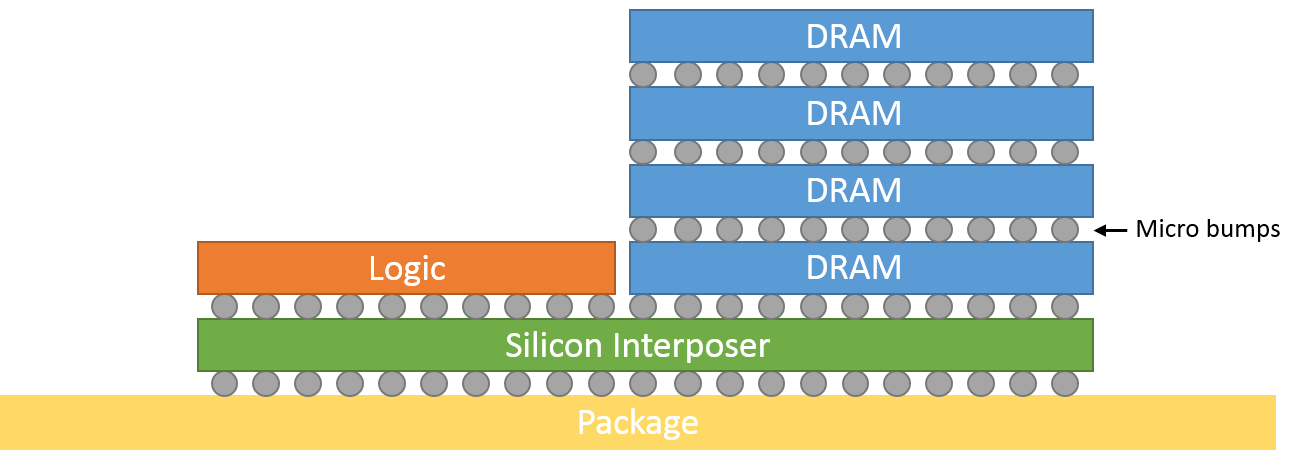
\includegraphics[width=0.75\linewidth]{figure/2D-integration.png}
\caption{Illustration of what a 2.5D chip might look like. The interposer is needed to enable communications between the Logic and DRAM. }
\label{2D-chip}
\end{figure}

\begin{figure}[!h]
\centering
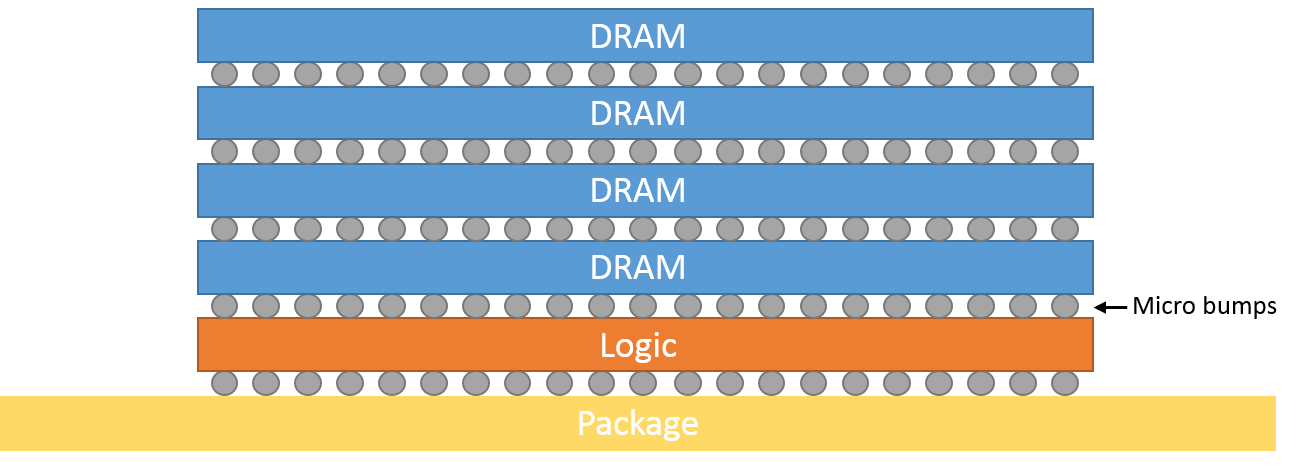
\includegraphics[width=0.75\linewidth]{figure/3D-integration.png}
\caption{Illustration of what a 3D chip might look like. All dies are directly connected through TSV.}
\label{3D-chip}
\end{figure}

Apart from introducing great potential in the future there are also some additional problems with stacking chips, e.g. verification and diverting thermal energy. There are several proposed methods of testing, where the underlying architecture could support both pre-bonding, mid-bonding and post-bonding tests. Pre-bonding tests are performed before and/or after doing wafer thinning, before dies are being stacked. When stacking, tests can be done on partial stacks, called mid-bond test, and complete stacks, called post-bond test. Testing after initial bonding could include creating additional test pins to form a Test Access Port \cite{Marinissen:2012:CES:2492708.2493023}, or creating special probe pads, due to the difficulties in probing micro-bumps without risking damaging them \cite{5751450}. Furthermore, high performance chips will inevitably lead to heat generation and by putting them  on top of one another the heat cannot easily dissipate; since the space between the dies are too small for air or liquid to pass efficiently, there need to be some other thermal cooling mechanism \cite{5501261}. The optimal thermal scenario is when the hottest chip is placed on top, nearest a heat spreader, which is inherently true when doing 2.5D integration. Having 3D chips makes it more complicated, but separating the most heat generating dies as much as possible minimizes in-package thermal transfer. This is one of several issues that has made 2.5D more realisable today, and still keeps 3D IC integration as a future goal. Due to the many advantages, performance-wise, with 3D stacking, it is very desirable to find a solution to this. Lastly, 3D stacking, compared to 2.5D, is also cheaper to manufacture because the package is smaller and less complex \cite{6263032}. This cost gap could, however, be lowered if the interposer die were to be tested before stacking, which could lead to an increased yield \cite{6542130}.
\bigskip

\section{Stacking memories}
TODO: While stacking can be done in several ways, there are a number of approaches to stacking only memories as well. Often memories are targeted for a specific integration method based on their architecture etc. 

There are a few noteworthy types of stacked memories: Hybrid Memory Cube (HMC), designed by Micron; High Bandwidth Memory (HBM), a JEDEC standard since 2013; and Wide-IO (WIO), also a JEDEC standard, since 2011. While the two former are designed for 2.5D integration -- memory on the same substrate as the processor -- the latter supports 2.5D, but is primarily aimed for 3D integration. TODO: Cite article stacking MRAM/STT-RAM as well to show that there are alternatives out there. TODO: Also mention that modern NAND flash today is stacked (3D- or V-NAND), used a lot. 
\bigskip

These memory technologies are all quite similar, but they primarily target different market segments. HMC is designed for high bandwidth at relatively high energy consumption and is comparatively expensive. This makes it more most suitable for High Performance Computing (HPC) systems. HBM was designed specifically for graphics applications, and there have been multiple commercial products (graphics cards) utilising this memory type in recent years. Similarly to HMC, this technology is made for systems where adequate cooling is available and where a higher cost can be somewhat overlooked. WIO on the other hand is architectured for being integrated on top of -- 3D integrated -- System on Chips (SoCs). These types of systems are generally found in mobile devices, which is also what WIO is designed for. Like HBM, WIO hopes to increase the performance of the graphics processors inside mobile devices. 
\bigskip

While these emerging types of memories are of interest on their own, whether they are non-volatile or standard DRAM, they could also be used in a Multi-Level Memory (MLM) design. An MLM design could utilise both the higher bandwidth of, e.g., HMC with the lower cost of DDR memory. A method has been described by Jayaraj et al. \cite{Jayaraj:2015:PPM:2818950.2818976}, where HMC is being used as a scratchpad type memory while DDR is still being used as main memory. This results in a higher performance while at a lower Bill of Materials (BoM) cost compared to a system using only DDR. However, the added cost of designing such a system is not included and not all applications are memory bound enough to benefit. Furthermore, it would also be necessary for software developers to optimise their applications for this setup in order to see any major gains \cite{Bender:2015:KCT:2818950.2818977}\cite{BENDER2017213}. TODO: If including PCM, mention multi-level memories here as well, with examples using PCM and DRAM buffers. Aka hybrid memory types.
\bigskip

%In the following chapters, we start off with the background of today's SDRAM memories and continue to explain how the emerging technologies operate. Then, we describe the different components, benchmark applications and simulators used in achieving the subsequent results. After that, we discuss the results and the implications they might have and finally give our conclusion. 